\chapter{Background}
% Studenten visar kännedom om teoretisk bakgrund och tidigare utfört arbete (betydande litteratur nämns och relevant material används).
% Bakgrunden är sammanhängande och relevant.
This Chapter will present background knowledge needed to comprehend conduction of the thesis. The chapter starts with a general description about \textit{\nameref{WebApplication}} structure and is followed by a section discussion common \textit{\nameref{SecurityVulnerabilities}} to web applications. After those follows two sections describing \textit{\nameref{DynamicTaintTracking}} and \textit{\nameref{DomainDrivenSecurity}}. The last section is a chapter about \textit{\nameref{JavaInstrumentation}}.


\section{Web Application}
\label{WebApplication}
To make applications available for large set of people and make them accessible from now days almost everywhere do businesses deploy their applications on the web. The deployment of an application can vary a lot but the most common structure for a web application is based on a three-tier architecture. The first tier is the presentation which is the visual components rendered by the browser. The second is the logic tire which is the brain of the application. The last and third tier is the storage, where the second tier can store data as needed \parencite{JustinClarke-Salt2009SIAa}. A illustration of the three layer architecture can be seen in figure \ref{fig:webApplication-Haldar}.

\begin{figure}
  \centering
  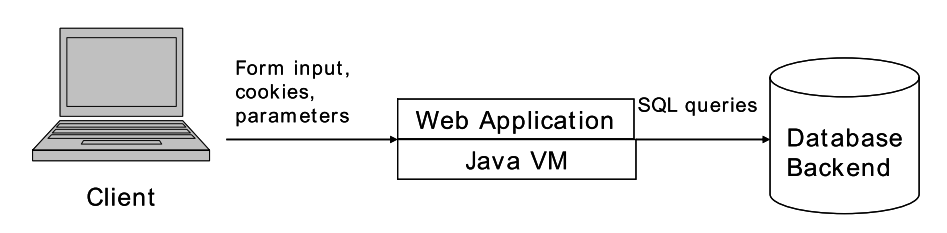
\includegraphics[width=\textwidth]{images/webApplication-Haldar.png}
  \caption{Web application architecture \cite{Haldar}.}
  \label{fig:webApplication-Haldar}
\end{figure}

It can be seen in figure \ref{fig:webApplication-Haldar} that the tiers only communicate with the tire closest to themselves. This causes the second tier to become a safe guard for tier three where the valuable and possibly sensitive information is stored. The storage tier contains all the information the application needs to provide the wanted service. Such information might for example be name, email, personal number and credit card information \parencite{JustinClarke-Salt2009SIAa}.

The scope of the thesis lies in tier two where the brain of the application lies. The programming language for tier two might vary a lot but one common and the chosen language for this thesis is Java.  


\subsection{Structured Query Language}
Communication between tier two and tier three is done through a standardize language called Structured Query Language, mostly known as SQL. SQL is created to anagrammatically manipulate and access databases. The clear majority of today's database uses SQL. The language works by building queries specifying the wanted information or task. The query will be evaluated and handled up upon by the SQL engine \parencite{DarieCristian2003TPGt}.


\section{Security Vulnerabilities}
\label{SecurityVulnerabilities}
The organization Open Web Applications Security Project, mostly known for its shortening (OWASP), is an online community which aim to provide knowledge how to secure web applications \parencite{OpenWebApplicationSecurityProject}. OWASP have produced reports about the top 10 security risks with a web application and the latest was published 2017. The report contains information about the ten most common application security risks that for the current year. Information such as how the security risk is exploited and possible prevention method is also presented. This thesis will look at security risk number one and eight which is Injection Attacks and Cross-site Scripting \parencite{OWASP2017}.


\subsection{CIA Triad}
Discussions about application security often relies on the CIA Triad which represent the three primary concepts in information security. These three are confidentiality, integrity and availability. Confidentiality are rules that specifies the access restrictions to the application. Integrity specifies that application data should be accurate and not altered. Availability is about ability to access the application and application data \parencite{2014C1-W}. This thesis focuses on confidentiality and integrity vulnerabilities and how we can prevent them.

\begin{figure}
  \centering
  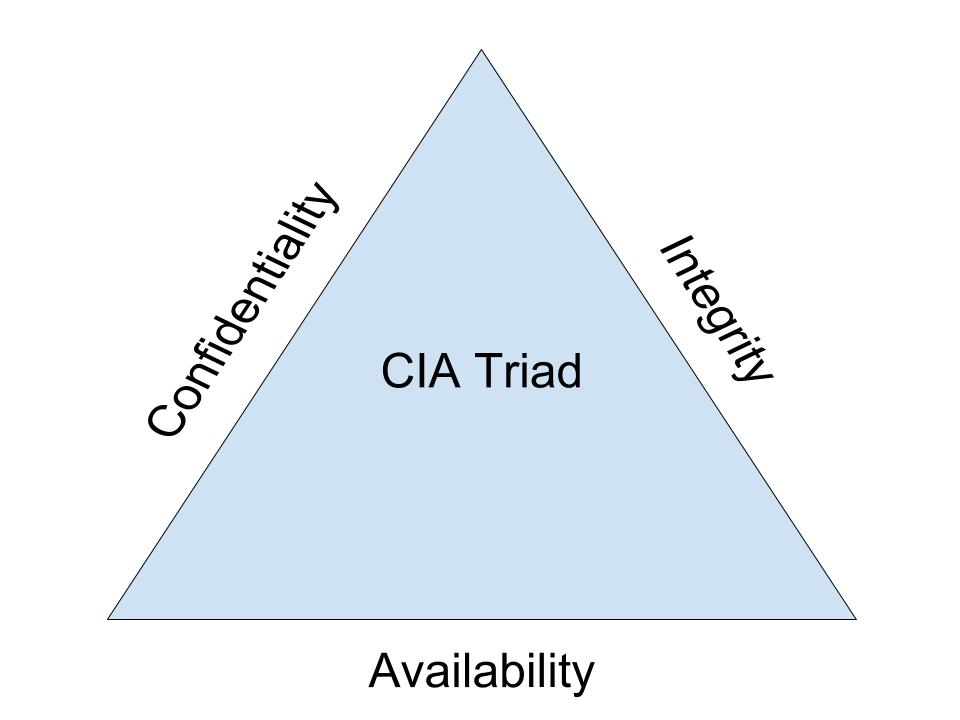
\includegraphics[height=6cm]{images/CIATriad.jpg}
  \caption{CIA Triad}
  \label{fig:CIATriad}
\end{figure}


\subsection{Injection}
The most common security risk is Injection Attacks \parencite{OWASP2017}. Injection Attack is any attack where the attacker's input changes the intent of the execution. Common result of Injection Attacks is file destruction, lack of accountability, denial of access and data loss \parencite{Secure_Web}.

Injection Attacks can be divided into two different subgroups. These two subgroups are SQL Injection and Blind SQL Injection \parencite{Secure_Web}.


\subsubsection{SQL Injection}
SQL Injection is when a SQL query is tampered which results in gaining content from the database which was not intended. Listing \ref{lst:acceptable_to_SQL_Injection} displays a SQL Query which is open to SQL Injections. This is due to the fact that the variable UserId is never validated before it is propagated into the query \parencite{JustinClarke-Salt2009SIAa, Secure_Web}.

\hfill
\begin{lstlisting}[
  language=SQL,
  caption=Code Acceptable to SQL Injection,
  label={lst:acceptable_to_SQL_Injection}]
userId = (*@\textit{userInput}@*)
"SELECT * FROM Users WHERE userId = " + userId
\end{lstlisting}
\hfill

The query will work as intended if the user input, notated with \textit{userInput}, only is a valid Integer (since Integer is what we have decided that user id is in this application). But what happens if the user input is \textit{10 or 1 = 1}? This user input would result in the query seen in listing \ref{lst:SQL_Injection}.

\hfill
\begin{lstlisting}[
  language=SQL,
  caption=SQL Injection,
  label={lst:SQL_Injection}]
SELECT * FROM Users WHERE userId = 10 or 1 = 1
\end{lstlisting}
\hfill

This query would result in query that always evaluates to true. The result of this will be that the query returns the whole table of users. This problem can be prevented in a couple of different ways. The first is through validation of the input. By verifying the input as seen in listing \ref{lst:SQL_Injection_Verified} can we protect the query from being assessable to SQL Injection.

\hfill
\begin{lstlisting}[
  language=SQL,
  caption=Preventing SQL Injection through Verification,
  label={lst:SQL_Injection_Verified}]
userId = (*@\textit{userInput}@*)
isInteger(userId)
"SELECT * FROM Users WHERE userId = " + userId
\end{lstlisting}
\hfill

A second more common alternative is to use SQL Parameters which handles the verification for the user. This leaves the verification and validation of input up to the SQL engine. An example written with SQL Parameters can be seen in listing \ref{lst:SQL_Injection_Parameters}.

\hfill
\begin{lstlisting}[
  language=SQL,
  caption=Preventing SQL Injection through SQL Parameters,
  label={lst:SQL_Injection_Parameters}]
userId = (*@\textit{userInput}@*)
sqlQuery = "SELECT * FROM Users WHERE userId = @0"
db.Execute(sqlQuery, userId)
\end{lstlisting}


\subsubsection{Blind SQL Injection}
Blind SQL Injection is very like SQL Injection. The only difference is that that attacker dose not receive the wanted information from the database. The information is instead received by monitoring variables such as how long time the response took or what kind of error messages it returns. An example of the first is a SQL query that tells the SQL engine to sleep depending on a condition. An example of this can be seen in listing \ref{lst:Blind_SQL_Injection_Time} \parencite{JustinClarke-Salt2009SIAa, Secure_Web}.

\hfill
\begin{lstlisting}[
  language=SQL,
  caption=Time Based Blind SQL Injection,
  label={lst:Blind_SQL_Injection_Time}]
SELECT * FROM Users WHERE userId = 1 WAITFOR DELAY '0:0:5'
\end{lstlisting}
\hfill

The second variant of Blind SQL Injection, which is by analysing the error messages, and depending on what they return build an image of the wanted answer. This is mostly done by testing different combination of true and false questions \parencite{JustinClarke-Salt2009SIAa, Secure_Web}.


\subsection{Cross-site Scripting}
Cross-Site Scripting (XSS) have been a vulnerability since the beginning of the internet. One of the first XSS attacks was created just after the release of JavaScript. The attack was conducted through loading a malicious web application into a frame on the site that the attacker want to gain information of. The attacker could then through JavaScript access any content that is visible or typed into the web application. To prevent this form of attack were the standard of Same-Origin Policy introduced. Same-Origin Policy restricts JavaScript to only access content from its own origin \parencite{FogieSeth2007Xacs, w3csop}.

But the introduction of the Same-Origin Policy did not stop the attackers from preforming XSS attacks. The next wave of attacks was mostly towards chat rooms where it was possible to inject malicious scripts into the input of the message. Which would then later be reflected by the server itself, when displaying the message for other users, and thereby bypassing the Same-Origin Policy \parencite{FogieSeth2007Xacs}.

XSS can be divided into three different sub categories. Which are: reflected, Stored and DOM Based XSS.

\subsubsection{Reflected XSS}
Reflected XSS is mostly conducted through a malicious link that an unknowing user clicks. The malicious link will exploit a vulnerable input on the targeted web application and though the input reflect back content to the user \parencite{Secure_Web}.


\subsubsection{Stored XSS}
Stored XSS is when malicious scripts are stored in the targeted web applications database. This malicious script is then loaded and presented for each user which is trying to access the application \parencite{Secure_Web}.


\subsubsection{DOM Based XSS}
DOM Based XSS is very similar to Reflected XSS but it does not necessary have to be reflected from the application server. DOM Based XSS modifies the DOM tree and can exploit the user \parencite{Secure_Web}.


\section{Dynamic Taint Tracking}
\label{DynamicTaintTracking}
Taint tracking, also known as taint analysis, taint checking and taint propagation, is a tool to analyse the flow of information in a domain \parencite{Pan2015}. the goal of taint tracking is to prevent possible attacks such as Injection Attacks and Cross-Site Scripting. Taint tracking can be done in two different ways: static and dynamic. The static is an evaluation tool which is done statically before runtime. Dynamic Taint Tracking is a tool that is executed in runtime. The tool works by tracking data in runtime and actively blocking any data that is trying to enter the sink without being detainted through validation first. Perl and Ruby are two programming languages which have adapted to user Taint checking \parencite{perl, ruby}. There are some tools who enables taint checking for other languages such as TaintDroid \parencite{Ma2010} and FlexTaint \parencite{Venkataramani2008}. This thesis will handle Dynamic Taint Checking and how it can increase the security of an application.

This is done by marking untrusted input from sources, which is a marking point where malicious data might enter the system, as tainted. This is done through a taint flag attached to the input. This taint flag follows the input throughout the application and propagates onto any other data it encounters. It is possible to detaint (remove the taint flag) tainted data but this is only done after the data have been sanitized through validation. The taint flags are checked in areas called sinks which are markings for entry points to sensitive code \parencite{Pan2015, Venkataramani2008}. The decision of what to do when a tainted variable try to pass through a sink might vary depending on the application. However, the common reaction is to stop the execution of the tainted code. Other actions such as logging or raising an alarm are also common. 
	
An example of taint tracking can be seen in listing \ref{lst:taint_propagation}. In this example \textit{getAttribute} is a source, \textit{executeQuery} a sink and \textit{validate} a sanitizer. On line one the input from the source is flagged tainted and the taint propagates onto \textit{userId}. The sanitizer on line two validates \textit{userId} and removes the taint flag. Lastly, the sink on line three execute since the argument is not tainted. If a user sends in a malicious userId containing "101 OR 1 = 1" the validator would either halt the execution or sanitize the String. However, removing line two would result in tainted data entering the sink. This would without a Dynamic Taint Tracking tool result in giving the malicious user the entire list of Users. With a Dynamic Taint Tracking tool however, would result in the sink halting the execution therefore preventing unwanted information disclosure.

\hfill
\begin{lstlisting}[
  caption=Taint Tracking,
  numbers=left,
  label={lst:taint_propagation}]
userId = getAttribute("userId");
validate(userId)
executeQuery("SELECT * FROM Users WHERE userId = " + userId);
\end{lstlisting}
\hfill

The above described Dynamic Taint Tracking tool focuses on preventing malicious code to enter the application. There are security policies restricting input from sources to pass through sinks without first being sanitized through validation. The same application could however be used to enforce policies restricting sensitive data from sinks to pass through sources without being sanitized to not contain sensitive data. 

This thesis will implement and evaluate a Dynamic Taint Tracking tool to prevent confidentiality and integrity vulnerabilities in web applications. The thesis will also evaluate the security benefits of Domain Driven Security, a programming paradigm which has been proposed to combat confidentiality and integrity vulnerabilities. Concretely, we will benchmark our Dynamic Taint Tracking tool against injection, cross-site scripting and information disclosure vulnerabilities.


\section{Domain Driven Security}
\label{DomainDrivenSecurity}
There exists a plethora of tools who aim to help in the process of developing complex domain models, but Domain Driven Design is not one of them \parencite{Bankes, 10.1007/978-3-319-24309-2_33}. Domain Driven Design is more of a thought process and methodology to follow every step of the process \parencite{EvansEric2004Dd:t}. In \emph{Domain-driven design reference: definitions and patterns summaries} do \textcite{evans_2015} describe Domain Driven Design through three core ideas:

\begin{itemize}
  \item Focus on the core domain.
  \item Explore models in a creative collaboration of domain practitioners and software practitioners.
  \item Speak a ubiquitous language within an explicitly bounded context.
\end{itemize}

The core domain is the part of your product that is most important and often is your main selling point compared to other similar products \parencite{millett_2015}. A discussion and even possible a documentation describing the core domain is something that will help the development of the product. The idea is to keep everybody on the same track heading in the same direction \parencite{EvansEric2004Dd:t}.

The second idea is to explore and develop every model in collaboration between domain practitioners, who are experts in the given domain, and software developers. This ensures that important knowledge needed to successfully develop the product is communicated back and forth between the two parties \parencite{millett_2015}. The third idea is important to enable and streamline the second. By using a ubiquitous language will miscommunication between domain and software practitioners be minimized and the collaboration between the two parties can instead focus on the important parts which is to develop the product \parencite{evans_2015}.

\textcite{evans_2015} do as well argue about the weight of clearly defining the bounded contexts for each defined model, and this needs to be done in the ubiquitous language created for the specific product. The need of this exists because of the otherwise great risk of misunderstandings and erroneous assumptions in the collaborations between the different models \parencite{millett_2015}.

\textcite{Wilander2009, Johnsson2009} created 2009 a blog post each in a synchronous manner where they together introduces the concept of Domain Driven Security to the public. They describe Domain Driven Security as the intersection between Domain Driven Design and application security. Domain Driven Design is about developing complex domain models and one of the most basic rule of application security is to always validate input data. Domain Driven Security in other hand, is about the importance of creating and maintaining domain models who are reflecting the product correctly and that they are validated so they can't be populated with erroneous data \parencite{Wilander2009, Johnsson2009, Arnor2016, Stendahl2016}.


\section{Java}
\label{JavaInstrumentation}
Java have been around since the early 90's. The founder's objective was to develop a new improved programming language that simplified the task for the developer but still had a familiar C/C++ syntax. \parencite{OracleVoice}. Today is Java one of the most common programming languages \parencite{octoverse}.

Java is a statically typed language which means that no variable can be used before they have been declared. These variables can be of two different types. These are primitives and references to objects. Among the primitives dose Java have support for eight. These are byte, short, int, long, float, double, boolean and char \parencite{primjav}.


\subsection{Java Virtual Machine}
There exists a plethora of implementation of the JVM but the official that Oracle develop is HotSpot \parencite{hotSpot}. One of the core ideas with Java during its development was "Write once, run anywhere". The slogan was created by Sun Microsystems which at the time were the company behind Java and the Java Virtual Machine, known as JVM. \parencite{Craig_2006}. The idea behind the JVM was to have one language that executed the same on all platforms. And then modify the JVM to be able to run on as many platforms as possible. The JVM is a virtual machine with its own components of heap storage, stack and program counter, method area and runtime constant pool. 

\begin{figure}
  \centering
  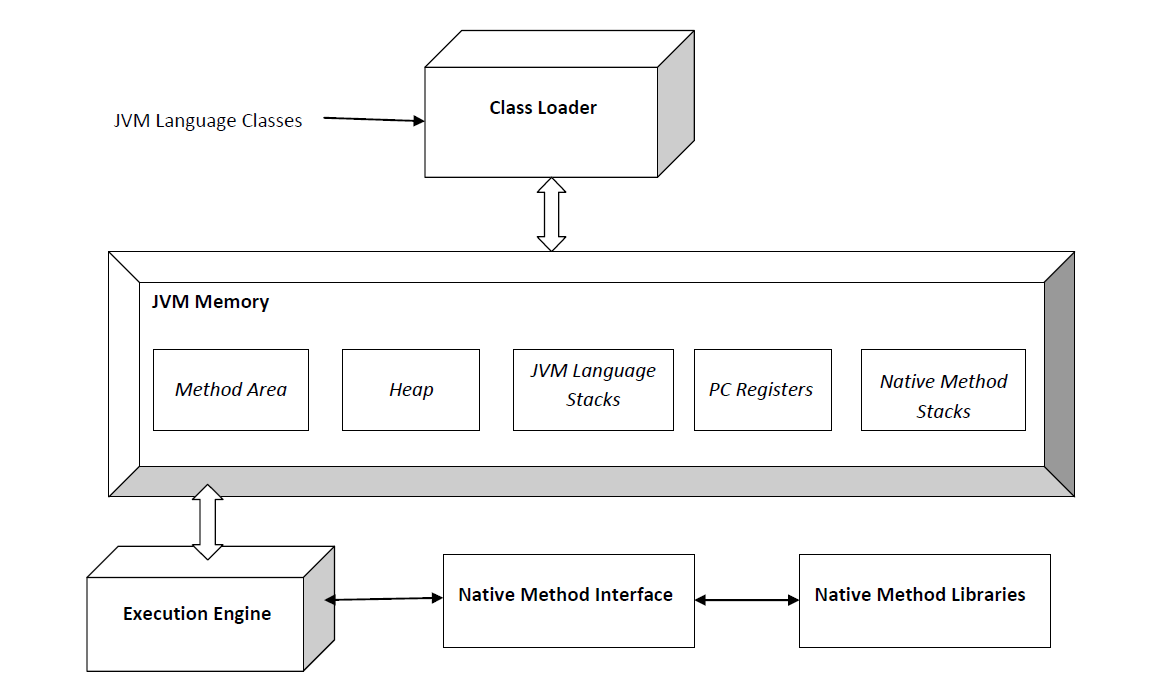
\includegraphics[width=\textwidth]{images/JvmSpec7.png}
  \caption{Java Virtual Machine Architecture}
  \label{fig:JVM}
\end{figure}

Figure \ref{fig:JVM} illustrates the architecture of the JVM. The compiled Java code that the developer creates is loaded through the Class Loader and added into the JVM Memory. \parencite{venners_1999}.


\subsection{Instrumentation}
Java Instrumentation is a way to modify the execution of an application on the Java Virtual Machine (JVM) without having knowledge nor the need of modifying the application code itself. This makes it beneficial to implement for example monitoring agents and event loggers through Java Instrumentation. Instrumentation is a Java package that provides services for modifying the bytecode of the program execution. Instrumentation works by implementing an Agent that will have the possibility to modify any application loaded in runtime \parencite{Java_Instrument}.


\subsection{Javassist}
There exist several libraries that can help the developer in the task of creating an Instrumentation Agent. The help comes in libraries of high level functions that later can be translated into bytecode that the JVM will understand. The library used in this thesis is Javassist. Javassist stands for Java programming Assistant and is a bytecode engineering toolkit. Javassist provides two levels of API where the one used in this thesis provides functionality of editing class files on source level which require no understanding of Java bytecode \parencite{Javassist}.